\let\negmedspace\undefined
\let\negthickspace\undefined
\documentclass[journal]{IEEEtran}
\usepackage[a5paper, margin=10mm, onecolumn]{geometry}
%\usepackage{lmodern} % Uncomment if needed for pdflatex
\usepackage{tfrupee} % Include tfrupee package

\setlength{\headheight}{1cm} % Set the height of the header box
\setlength{\headsep}{0mm}     % Set the distance between the header box and the top of the text

\usepackage{gvv-book}
\usepackage{gvv}
\usepackage{cite}
\usepackage{amsmath,amssymb,amsfonts,amsthm}
\usepackage{algorithmic}
\usepackage{graphicx}
\usepackage{textcomp}
\usepackage{xcolor}
\usepackage{txfonts}
\usepackage{listings}
\usepackage{enumitem}
\usepackage{mathtools}
\usepackage{gensymb}
\usepackage{comment}
\usepackage[breaklinks=true]{hyperref}
\usepackage{tkz-euclide} 
\usepackage{listings}
%\usepackage{gvv}                                        
\def\inputGnumericTable{}                                 
\usepackage[latin1]{inputenc}                                
\usepackage{color}                                            
\usepackage{array}                                            
\usepackage{longtable}                                       
\usepackage{calc}                                             
\usepackage{multirow}                                         
\usepackage{hhline}                                           
\usepackage{ifthen}                                           
\usepackage{lscape}
\usepackage{tikz}
\usepackage{circuitikz}
\usepackage{standalone} % For including external TikZ files

\begin{document}

\bibliographystyle{IEEEtran}
\vspace{3cm}

\title{6.5.2.2}
\author{EE24BTECH11066 - YERRA AKHILESH}
% \maketitle
% \newpage
% \bigskip
{\let\newpage\relax\maketitle}

\renewcommand{\thefigure}{\theenumi}
\renewcommand{\thetable}{\theenumi}
\setlength{\intextsep}{10pt} % Space between text and floats

\numberwithin{equation}{enumi}
\numberwithin{figure}{enumi}
\renewcommand{\thetable}{\theenumi}
\textbf{Question}:\\
Find the Maximum and Minimum values of the function \\
$$y(x) = - \abs{x + 1} +3$$\\
\textbf{Solution : }\\
\textbf{Threotical Solution :}\\

As $y(x)$ is modular function, The vertex of the function is at the point where,
\begin{align}
    \abs{x + 1} = 0\\
    x = -1
\end{align}
Substitute $x = -1$ in the function, gives :
\begin{align}
    y(-1) = 3
\end{align}
Hence, the vertex is at $\brak{-1,3}$, which is the \textbf{maximum} point and it can be explained by ,
$$y =
\begin{cases} 
-(x+1) + 3 & \text{if } x \geq -1, \\ 
(x+1) + 3 & \text{if } x < -1
\end{cases}
$$
The derivative of $y$ is:
$$
\frac{dy}{dx} =
\begin{cases} 
-1 & \text{if } x > -1, \\ 
1 & \text{if } x < -1.
\end{cases}
$$
At $x = -1$, the derivative does not exist because of the abrupt change in slope. However, we can observe the behavior of the function:\\
- For  $x < -1$, the derivative $\frac{dy}{dx} = 1 > 0$, indicating that the function is increasing.\\
- For $x > -1$, the derivative $\frac{dy}{dx} = -1 < 0$, indicating that the function is decreasing.\\

Therefore, \textbf{maximum} value of $y(x) = 3$  at $x = -1$ \\


Now,\\
As $x \rightarrow \infty$ or $x \rightarrow -\infty$, the absolute value $\abs{x+1} \rightarrow \infty$, and the negative of this term dominates. Thus:
\begin{align}
    y \rightarrow -\infty
\end{align}
This means the function decreases without bound, so there \textbf{is no minimum value.}\\


\textbf{Computational solution :}\\
Maximum value of the function can be done by \textbf{Gradient Ascent} method:
\begin{itemize}
    \item \textbf{Choose a starting point} - $x_0$ away from $x = -1$.
    \item \textbf{Update the position iteratively}:
    $$x_{n+1} = x_{n} + \eta \cdot \frac{dy}{dx}$$\\
    Here, $\eta = 0.01$, $\eta$ is learning rate.
    \item \textbf{Behaviour in each region}:\\
    \textbf{for $x > -1$}:   $\frac{dy}{dx} = -1$,
    \begin{align}
        x_{n+1} = x_{n} - \eta
    \end{align}
    This causes $x_n$ to decrease toward $x = -1$.\\
    \textbf{for} $x < -1$: $\frac{dy}{dx} = 1$,
    \begin{align}
        x_{n+1} = x_{n} + \eta
    \end{align}
    This causes $x_n$ to increase toward $x = -1$.\\
\textbf{At} $x = -1$:  \\
the gradient changes direction abruptly, and the iteration stops because the function value is maximized at this point.
\end{itemize}
Minimum value of the function can be done by \textbf{Gradient decent} method:\\

Here,
\begin{align}
    x_{n+1} = x_{n} - \eta \cdot \frac{dy}{dx}
\end{align}

\textbf{Similarly finding behaviour in each region}:\\
\textbf{for} $x>-1$: \\
\begin{align}
    x_{n+1} = x_{n} + \eta
\end{align}
This causes $x_n$ to increase indefinitely, moving away from $x = -1$.\\
\textbf{for} $x<-1$: \\
\begin{align}
    x_{n+1} = x_{n} - \eta
\end{align}
This causes $x_n$ to decrease indefinitely, moving away from $x = -1$.\\ 

The function decreases without bound as $x \rightarrow \infty$ or $x \rightarrow -\infty$, so \textbf{gradient descent} will not converge to a minimum. The iteration will continue indefinitely.
so, \textbf{No Minimum exists}\\

\textbf{Computational results :}\\
-Absolute Maximum
\begin{align}
    x \approx -1 , \text{ } y(x) \approx 3  
\end{align}
-No Absolute Minimum\\

 \begin{figure}[ht!]
   \centering
   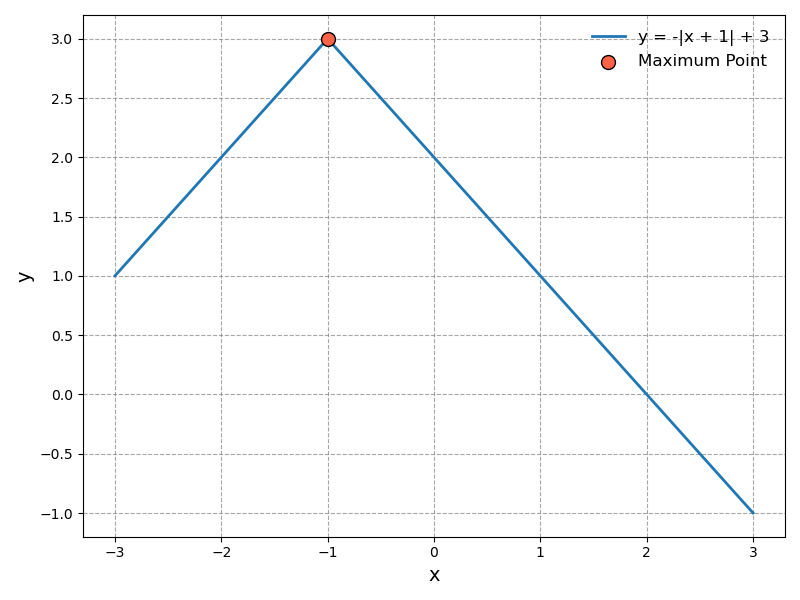
\includegraphics[width=\columnwidth]{figs/Figure_1.png}
\end{figure}
\end{document}
